
\begin{frame}{Disseny d'un model pels SGBD Round Robin}
  Una base de dades Round Robin és un contenidor informàtic d'una
  sèrie temporal que prové d'un monitoratge d'una variable mesurada en
  diferents instants de temps.

  \begin{enumerate}

  \item Mesura $m=(v,t)$. %Valor en un instant temps.
    \begin{itemize}
    \item Les mesures tenen relació d'ordre induïda pel temps.
    \end{itemize}

  \item Sèrie temporal $S=\{m_0,\ldots,m_k\}$. %Conjunt de mesures.
    \begin{itemize}
    \item Regular si les mesures són equidistants en el temps.
    \end{itemize}

  \item Buffer $B=(S,\tau,\delta,f)$. %Consolidació d'una sèrie temporal.
    \begin{itemize}
    \item \emph{afegeix}: $B \times m \mapsto B'$.
    \item \emph{consolida}: $B \mapsto B' \times m'$.
    \item $\delta$ pas de consolidació
    \item $\tau$ darrer instant de consolidació.
    \item Interpolació $f: S \times [\tau,\tau+\delta] \mapsto m'$.
    \end{itemize}

  \item Disc $D=(S,k)$. 
    \begin{itemize}
    \item Emmagatzematge acotat: $|S| \leq k$. 
    \item \emph{afegeix}: $D \times m \mapsto D'$.
    \end{itemize}

  \end{enumerate}

\begin{textblock*}{50mm}(70mm,-40mm)

%\column{5cm}
  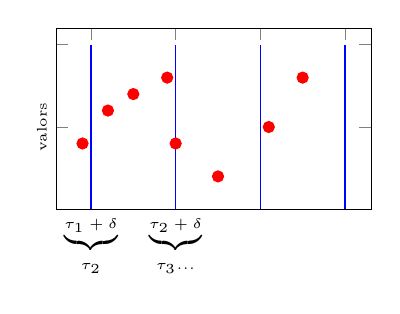
\begin{tikzpicture}
    \begin{axis}[
        width=4cm,
        scale only axis, height=2.3cm,
        ymin = 0,
        yticklabels= {,,\tiny valors},
        y tick label style = {rotate=90,anchor=south},
        x tick label style = {font=\tiny},        
        xticklabels={$\underbrace{\tau_{}}_{\tau_0}$,$\underbrace{\tau_0+\delta}_{\tau_1}$,$\underbrace{\tau_1+\delta}_{\tau_2}$,$\underbrace{\tau_2+\delta}_{\tau_3 \ldots}$},
        ]
 
    \addplot[ycomb,blue] coordinates {
        (20,10)
        (30,10)
        (40,10)
        (50,10)
    }; 

    \addplot[red,only marks, mark = *] coordinates {
        (19,4)
        (22,6)
        (25,7)
        (29,8)
        (30,4)
        (35,2)
        (41,5)
        (45,8)
    };

    \end{axis}
  \end{tikzpicture}


\end{textblock*}


%\end{columns}

\end{frame}


\begin{frame}{Model RRD: esquema de funcionament}

\begin{enumerate}
\setcounter{enumi}{4}
\item Disc Round Robin $R=(B,D)$. 
\begin{itemize}
\item Consolidació de buffer a disc.
\end{itemize}
\item Base de dades Round Robin $M=(B,\{R_0,\ldots,R_d \})$. 
\begin{itemize}
\item Sèrie temporal compacta i repartida en discs Round Robin:
\end{itemize}
\end{enumerate}



  % \begin{columns}[l]
  %    \column{6cm}

\begin{center}
       \tiny
       \setlength{\unitlength}{0.2mm}
       % Graphic for TeX using PGF
% Title: /home/aleix/pfc_svn/imatges/model/arxiurrd.dia
% Creator: Dia v0.97.1
% CreationDate: Tue May 31 13:01:29 2011
% For: aleix
% \usepackage{tikz}
% The following commands are not supported in PSTricks at present
% We define them conditionally, so when they are implemented,
% this pgf file will use them.
\ifx\du\undefined
  \newlength{\du}
\fi
\setlength{\du}{15\unitlength}
\begin{tikzpicture}
\pgftransformxscale{1.000000}
\pgftransformyscale{-1.000000}
\definecolor{dialinecolor}{rgb}{0.000000, 0.000000, 0.000000}
\pgfsetstrokecolor{dialinecolor}
\definecolor{dialinecolor}{rgb}{1.000000, 1.000000, 1.000000}
\pgfsetfillcolor{dialinecolor}
\definecolor{dialinecolor}{rgb}{1.000000, 1.000000, 1.000000}
\pgfsetfillcolor{dialinecolor}
\fill (7.200000\du,-9.403364\du)--(7.200000\du,4.396636\du)--(28.200000\du,4.396636\du)--(28.200000\du,-9.403364\du)--cycle;
\pgfsetlinewidth{0.100000\du}
\pgfsetdash{}{0pt}
\pgfsetdash{}{0pt}
\pgfsetmiterjoin
\definecolor{dialinecolor}{rgb}{0.000000, 0.000000, 0.000000}
\pgfsetstrokecolor{dialinecolor}
\draw (7.200000\du,-9.403364\du)--(7.200000\du,4.396636\du)--(28.200000\du,4.396636\du)--(28.200000\du,-9.403364\du)--cycle;
% setfont left to latex
\definecolor{dialinecolor}{rgb}{0.000000, 0.000000, 0.000000}
\pgfsetstrokecolor{dialinecolor}
\node at (17.700000\du,-2.308364\du){};
\definecolor{dialinecolor}{rgb}{1.000000, 1.000000, 1.000000}
\pgfsetfillcolor{dialinecolor}
\pgfpathellipse{\pgfpoint{11.767338\du}{-0.851682\du}}{\pgfpoint{3.224066\du}{0\du}}{\pgfpoint{0\du}{3.826682\du}}
\pgfusepath{fill}
\pgfsetlinewidth{0.100000\du}
\pgfsetdash{}{0pt}
\pgfsetdash{}{0pt}
\pgfsetmiterjoin
\definecolor{dialinecolor}{rgb}{0.000000, 0.000000, 0.000000}
\pgfsetstrokecolor{dialinecolor}
\pgfpathellipse{\pgfpoint{11.767338\du}{-0.851682\du}}{\pgfpoint{3.224066\du}{0\du}}{\pgfpoint{0\du}{3.826682\du}}
\pgfusepath{stroke}
% setfont left to latex
\definecolor{dialinecolor}{rgb}{0.000000, 0.000000, 0.000000}
\pgfsetstrokecolor{dialinecolor}
\node at (11.767338\du,-0.656682\du){};
\definecolor{dialinecolor}{rgb}{1.000000, 1.000000, 1.000000}
\pgfsetfillcolor{dialinecolor}
\pgfpathellipse{\pgfpoint{11.746636\du}{1.048318\du}}{\pgfpoint{1.403364\du}{0\du}}{\pgfpoint{0\du}{1.376682\du}}
\pgfusepath{fill}
\pgfsetlinewidth{0.100000\du}
\pgfsetdash{}{0pt}
\pgfsetdash{}{0pt}
\pgfsetmiterjoin
\definecolor{dialinecolor}{rgb}{0.000000, 0.000000, 0.000000}
\pgfsetstrokecolor{dialinecolor}
\pgfpathellipse{\pgfpoint{11.746636\du}{1.048318\du}}{\pgfpoint{1.403364\du}{0\du}}{\pgfpoint{0\du}{1.376682\du}}
\pgfusepath{stroke}
% setfont left to latex
\definecolor{dialinecolor}{rgb}{0.000000, 0.000000, 0.000000}
\pgfsetstrokecolor{dialinecolor}
\node at (11.746636\du,1.243318\du){};
\pgfsetlinewidth{0.100000\du}
\pgfsetdash{}{0pt}
\pgfsetdash{}{0pt}
\pgfsetbuttcap
\pgfsetmiterjoin
\pgfsetlinewidth{0.100000\du}
\pgfsetbuttcap
\pgfsetmiterjoin
\pgfsetdash{}{0pt}
\definecolor{dialinecolor}{rgb}{1.000000, 1.000000, 1.000000}
\pgfsetfillcolor{dialinecolor}
\pgfpathmoveto{\pgfpoint{10.850000\du}{-3.858333\du}}
\pgfpathcurveto{\pgfpoint{11.250000\du}{-4.152083\du}}{\pgfpoint{11.450000\du}{-4.250000\du}}{\pgfpoint{11.850000\du}{-4.250000\du}}
\pgfpathcurveto{\pgfpoint{12.250000\du}{-4.250000\du}}{\pgfpoint{12.450000\du}{-4.152083\du}}{\pgfpoint{12.850000\du}{-3.858333\du}}
\pgfpathlineto{\pgfpoint{12.850000\du}{-2.291667\du}}
\pgfpathcurveto{\pgfpoint{12.450000\du}{-1.997917\du}}{\pgfpoint{12.250000\du}{-1.900000\du}}{\pgfpoint{11.850000\du}{-1.900000\du}}
\pgfpathcurveto{\pgfpoint{11.450000\du}{-1.900000\du}}{\pgfpoint{11.250000\du}{-1.997917\du}}{\pgfpoint{10.850000\du}{-2.291667\du}}
\pgfpathlineto{\pgfpoint{10.850000\du}{-3.858333\du}}
\pgfusepath{fill}
\definecolor{dialinecolor}{rgb}{0.000000, 0.000000, 0.000000}
\pgfsetstrokecolor{dialinecolor}
\pgfpathmoveto{\pgfpoint{10.850000\du}{-3.858333\du}}
\pgfpathcurveto{\pgfpoint{11.250000\du}{-4.152083\du}}{\pgfpoint{11.450000\du}{-4.250000\du}}{\pgfpoint{11.850000\du}{-4.250000\du}}
\pgfpathcurveto{\pgfpoint{12.250000\du}{-4.250000\du}}{\pgfpoint{12.450000\du}{-4.152083\du}}{\pgfpoint{12.850000\du}{-3.858333\du}}
\pgfpathlineto{\pgfpoint{12.850000\du}{-2.291667\du}}
\pgfpathcurveto{\pgfpoint{12.450000\du}{-1.997917\du}}{\pgfpoint{12.250000\du}{-1.900000\du}}{\pgfpoint{11.850000\du}{-1.900000\du}}
\pgfpathcurveto{\pgfpoint{11.450000\du}{-1.900000\du}}{\pgfpoint{11.250000\du}{-1.997917\du}}{\pgfpoint{10.850000\du}{-2.291667\du}}
\pgfpathlineto{\pgfpoint{10.850000\du}{-3.858333\du}}
\pgfusepath{stroke}
\pgfsetbuttcap
\pgfsetmiterjoin
\pgfsetdash{}{0pt}
\definecolor{dialinecolor}{rgb}{0.000000, 0.000000, 0.000000}
\pgfsetstrokecolor{dialinecolor}
\pgfpathmoveto{\pgfpoint{10.850000\du}{-3.858333\du}}
\pgfpathcurveto{\pgfpoint{11.250000\du}{-3.564583\du}}{\pgfpoint{11.450000\du}{-3.466667\du}}{\pgfpoint{11.850000\du}{-3.466667\du}}
\pgfpathcurveto{\pgfpoint{12.250000\du}{-3.466667\du}}{\pgfpoint{12.450000\du}{-3.564583\du}}{\pgfpoint{12.850000\du}{-3.858333\du}}
\pgfusepath{stroke}
% setfont left to latex
\definecolor{dialinecolor}{rgb}{0.000000, 0.000000, 0.000000}
\pgfsetstrokecolor{dialinecolor}
\node at (11.850000\du,-2.679167\du){};
\pgfsetlinewidth{0.100000\du}
\pgfsetdash{}{0pt}
\pgfsetdash{}{0pt}
\pgfsetbuttcap
{
\definecolor{dialinecolor}{rgb}{0.000000, 0.000000, 0.000000}
\pgfsetfillcolor{dialinecolor}
% was here!!!
\definecolor{dialinecolor}{rgb}{0.000000, 0.000000, 0.000000}
\pgfsetstrokecolor{dialinecolor}
\pgfpathmoveto{\pgfpoint{12.471610\du}{1.123386\du}}
\pgfpatharc{21}{-200}{0.737486\du and 0.737486\du}
\pgfusepath{stroke}
}
\pgfsetlinewidth{0.100000\du}
\pgfsetdash{}{0pt}
\pgfsetdash{}{0pt}
\pgfsetbuttcap
{
\definecolor{dialinecolor}{rgb}{0.000000, 0.000000, 0.000000}
\pgfsetfillcolor{dialinecolor}
% was here!!!
\definecolor{dialinecolor}{rgb}{0.000000, 0.000000, 0.000000}
\pgfsetstrokecolor{dialinecolor}
\draw (16.171636\du,0.473318\du)--(16.171636\du,0.473318\du);
}
\pgfsetlinewidth{0.100000\du}
\pgfsetdash{}{0pt}
\pgfsetdash{}{0pt}
\pgfsetbuttcap
{
\definecolor{dialinecolor}{rgb}{0.000000, 0.000000, 0.000000}
\pgfsetfillcolor{dialinecolor}
% was here!!!
\definecolor{dialinecolor}{rgb}{0.000000, 0.000000, 0.000000}
\pgfsetstrokecolor{dialinecolor}
\draw (11.200000\du,1.125000\du)--(10.800000\du,0.825000\du);
}
\pgfsetlinewidth{0.100000\du}
\pgfsetdash{}{0pt}
\pgfsetdash{}{0pt}
\pgfsetbuttcap
{
\definecolor{dialinecolor}{rgb}{0.000000, 0.000000, 0.000000}
\pgfsetfillcolor{dialinecolor}
% was here!!!
\definecolor{dialinecolor}{rgb}{0.000000, 0.000000, 0.000000}
\pgfsetstrokecolor{dialinecolor}
\draw (11.150000\du,1.075000\du)--(11.500000\du,0.825000\du);
}
\pgfsetlinewidth{0.100000\du}
\pgfsetdash{}{0pt}
\pgfsetdash{}{0pt}
\pgfsetbuttcap
{
\definecolor{dialinecolor}{rgb}{0.000000, 0.000000, 0.000000}
\pgfsetfillcolor{dialinecolor}
% was here!!!
\pgfsetarrowsend{to}
\definecolor{dialinecolor}{rgb}{0.000000, 0.000000, 0.000000}
\pgfsetstrokecolor{dialinecolor}
\draw (11.819301\du,-1.850387\du)--(11.782382\du,-0.377629\du);
}
% setfont left to latex
\definecolor{dialinecolor}{rgb}{0.000000, 0.000000, 0.000000}
\pgfsetstrokecolor{dialinecolor}
\node[anchor=west] at (10.950000\du,-2.625000\du){buffer};
% setfont left to latex
\definecolor{dialinecolor}{rgb}{0.000000, 0.000000, 0.000000}
\pgfsetstrokecolor{dialinecolor}
\node[anchor=west] at (11.246636\du,1.748318\du){disc};
% setfont left to latex
\definecolor{dialinecolor}{rgb}{0.000000, 0.000000, 0.000000}
\pgfsetstrokecolor{dialinecolor}
\node[anchor=west] at (9.067338\du,3.548318\du){disc Round Robin};
\definecolor{dialinecolor}{rgb}{1.000000, 1.000000, 1.000000}
\pgfsetfillcolor{dialinecolor}
\pgfpathellipse{\pgfpoint{23.469066\du}{-0.783318\du}}{\pgfpoint{3.224066\du}{0\du}}{\pgfpoint{0\du}{3.826682\du}}
\pgfusepath{fill}
\pgfsetlinewidth{0.100000\du}
\pgfsetdash{}{0pt}
\pgfsetdash{}{0pt}
\pgfsetmiterjoin
\definecolor{dialinecolor}{rgb}{0.000000, 0.000000, 0.000000}
\pgfsetstrokecolor{dialinecolor}
\pgfpathellipse{\pgfpoint{23.469066\du}{-0.783318\du}}{\pgfpoint{3.224066\du}{0\du}}{\pgfpoint{0\du}{3.826682\du}}
\pgfusepath{stroke}
% setfont left to latex
\definecolor{dialinecolor}{rgb}{0.000000, 0.000000, 0.000000}
\pgfsetstrokecolor{dialinecolor}
\node at (23.469066\du,-0.588318\du){};
\definecolor{dialinecolor}{rgb}{1.000000, 1.000000, 1.000000}
\pgfsetfillcolor{dialinecolor}
\pgfpathellipse{\pgfpoint{23.448364\du}{1.116682\du}}{\pgfpoint{1.403364\du}{0\du}}{\pgfpoint{0\du}{1.376682\du}}
\pgfusepath{fill}
\pgfsetlinewidth{0.100000\du}
\pgfsetdash{}{0pt}
\pgfsetdash{}{0pt}
\pgfsetmiterjoin
\definecolor{dialinecolor}{rgb}{0.000000, 0.000000, 0.000000}
\pgfsetstrokecolor{dialinecolor}
\pgfpathellipse{\pgfpoint{23.448364\du}{1.116682\du}}{\pgfpoint{1.403364\du}{0\du}}{\pgfpoint{0\du}{1.376682\du}}
\pgfusepath{stroke}
% setfont left to latex
\definecolor{dialinecolor}{rgb}{0.000000, 0.000000, 0.000000}
\pgfsetstrokecolor{dialinecolor}
\node at (23.448364\du,1.311682\du){};
\pgfsetlinewidth{0.100000\du}
\pgfsetdash{}{0pt}
\pgfsetdash{}{0pt}
\pgfsetbuttcap
\pgfsetmiterjoin
\pgfsetlinewidth{0.100000\du}
\pgfsetbuttcap
\pgfsetmiterjoin
\pgfsetdash{}{0pt}
\definecolor{dialinecolor}{rgb}{1.000000, 1.000000, 1.000000}
\pgfsetfillcolor{dialinecolor}
\pgfpathmoveto{\pgfpoint{22.551728\du}{-3.789969\du}}
\pgfpathcurveto{\pgfpoint{22.951728\du}{-4.083719\du}}{\pgfpoint{23.151728\du}{-4.181636\du}}{\pgfpoint{23.551728\du}{-4.181636\du}}
\pgfpathcurveto{\pgfpoint{23.951728\du}{-4.181636\du}}{\pgfpoint{24.151728\du}{-4.083719\du}}{\pgfpoint{24.551728\du}{-3.789969\du}}
\pgfpathlineto{\pgfpoint{24.551728\du}{-2.223303\du}}
\pgfpathcurveto{\pgfpoint{24.151728\du}{-1.929553\du}}{\pgfpoint{23.951728\du}{-1.831636\du}}{\pgfpoint{23.551728\du}{-1.831636\du}}
\pgfpathcurveto{\pgfpoint{23.151728\du}{-1.831636\du}}{\pgfpoint{22.951728\du}{-1.929553\du}}{\pgfpoint{22.551728\du}{-2.223303\du}}
\pgfpathlineto{\pgfpoint{22.551728\du}{-3.789969\du}}
\pgfusepath{fill}
\definecolor{dialinecolor}{rgb}{0.000000, 0.000000, 0.000000}
\pgfsetstrokecolor{dialinecolor}
\pgfpathmoveto{\pgfpoint{22.551728\du}{-3.789969\du}}
\pgfpathcurveto{\pgfpoint{22.951728\du}{-4.083719\du}}{\pgfpoint{23.151728\du}{-4.181636\du}}{\pgfpoint{23.551728\du}{-4.181636\du}}
\pgfpathcurveto{\pgfpoint{23.951728\du}{-4.181636\du}}{\pgfpoint{24.151728\du}{-4.083719\du}}{\pgfpoint{24.551728\du}{-3.789969\du}}
\pgfpathlineto{\pgfpoint{24.551728\du}{-2.223303\du}}
\pgfpathcurveto{\pgfpoint{24.151728\du}{-1.929553\du}}{\pgfpoint{23.951728\du}{-1.831636\du}}{\pgfpoint{23.551728\du}{-1.831636\du}}
\pgfpathcurveto{\pgfpoint{23.151728\du}{-1.831636\du}}{\pgfpoint{22.951728\du}{-1.929553\du}}{\pgfpoint{22.551728\du}{-2.223303\du}}
\pgfpathlineto{\pgfpoint{22.551728\du}{-3.789969\du}}
\pgfusepath{stroke}
\pgfsetbuttcap
\pgfsetmiterjoin
\pgfsetdash{}{0pt}
\definecolor{dialinecolor}{rgb}{0.000000, 0.000000, 0.000000}
\pgfsetstrokecolor{dialinecolor}
\pgfpathmoveto{\pgfpoint{22.551728\du}{-3.789969\du}}
\pgfpathcurveto{\pgfpoint{22.951728\du}{-3.496219\du}}{\pgfpoint{23.151728\du}{-3.398303\du}}{\pgfpoint{23.551728\du}{-3.398303\du}}
\pgfpathcurveto{\pgfpoint{23.951728\du}{-3.398303\du}}{\pgfpoint{24.151728\du}{-3.496219\du}}{\pgfpoint{24.551728\du}{-3.789969\du}}
\pgfusepath{stroke}
% setfont left to latex
\definecolor{dialinecolor}{rgb}{0.000000, 0.000000, 0.000000}
\pgfsetstrokecolor{dialinecolor}
\node at (23.551728\du,-2.610803\du){};
\pgfsetlinewidth{0.100000\du}
\pgfsetdash{}{0pt}
\pgfsetdash{}{0pt}
\pgfsetbuttcap
{
\definecolor{dialinecolor}{rgb}{0.000000, 0.000000, 0.000000}
\pgfsetfillcolor{dialinecolor}
% was here!!!
\definecolor{dialinecolor}{rgb}{0.000000, 0.000000, 0.000000}
\pgfsetstrokecolor{dialinecolor}
\pgfpathmoveto{\pgfpoint{24.173338\du}{1.191750\du}}
\pgfpatharc{21}{-200}{0.737486\du and 0.737486\du}
\pgfusepath{stroke}
}
\pgfsetlinewidth{0.100000\du}
\pgfsetdash{}{0pt}
\pgfsetdash{}{0pt}
\pgfsetbuttcap
{
\definecolor{dialinecolor}{rgb}{0.000000, 0.000000, 0.000000}
\pgfsetfillcolor{dialinecolor}
% was here!!!
\definecolor{dialinecolor}{rgb}{0.000000, 0.000000, 0.000000}
\pgfsetstrokecolor{dialinecolor}
\draw (27.873364\du,0.541682\du)--(27.873364\du,0.541682\du);
}
\pgfsetlinewidth{0.100000\du}
\pgfsetdash{}{0pt}
\pgfsetdash{}{0pt}
\pgfsetbuttcap
{
\definecolor{dialinecolor}{rgb}{0.000000, 0.000000, 0.000000}
\pgfsetfillcolor{dialinecolor}
% was here!!!
\definecolor{dialinecolor}{rgb}{0.000000, 0.000000, 0.000000}
\pgfsetstrokecolor{dialinecolor}
\draw (22.901728\du,1.193364\du)--(22.501728\du,0.893364\du);
}
\pgfsetlinewidth{0.100000\du}
\pgfsetdash{}{0pt}
\pgfsetdash{}{0pt}
\pgfsetbuttcap
{
\definecolor{dialinecolor}{rgb}{0.000000, 0.000000, 0.000000}
\pgfsetfillcolor{dialinecolor}
% was here!!!
\definecolor{dialinecolor}{rgb}{0.000000, 0.000000, 0.000000}
\pgfsetstrokecolor{dialinecolor}
\draw (22.851728\du,1.143364\du)--(23.201728\du,0.893364\du);
}
\pgfsetlinewidth{0.100000\du}
\pgfsetdash{}{0pt}
\pgfsetdash{}{0pt}
\pgfsetbuttcap
{
\definecolor{dialinecolor}{rgb}{0.000000, 0.000000, 0.000000}
\pgfsetfillcolor{dialinecolor}
% was here!!!
\pgfsetarrowsend{to}
\definecolor{dialinecolor}{rgb}{0.000000, 0.000000, 0.000000}
\pgfsetstrokecolor{dialinecolor}
\draw (23.521029\du,-1.782023\du)--(23.484110\du,-0.309265\du);
}
% setfont left to latex
\definecolor{dialinecolor}{rgb}{0.000000, 0.000000, 0.000000}
\pgfsetstrokecolor{dialinecolor}
\node[anchor=west] at (22.651728\du,-2.556636\du){buffer};
% setfont left to latex
\definecolor{dialinecolor}{rgb}{0.000000, 0.000000, 0.000000}
\pgfsetstrokecolor{dialinecolor}
\node[anchor=west] at (22.948364\du,1.816682\du){disc};
% setfont left to latex
\definecolor{dialinecolor}{rgb}{0.000000, 0.000000, 0.000000}
\pgfsetstrokecolor{dialinecolor}
\node[anchor=west] at (20.769066\du,3.616682\du){disc Round Robin};
% setfont left to latex
\definecolor{dialinecolor}{rgb}{0.000000, 0.000000, 0.000000}
\pgfsetstrokecolor{dialinecolor}
\node[anchor=west] at (17.450000\du,-0.950000\du){...};
% setfont left to latex
\definecolor{dialinecolor}{rgb}{0.000000, 0.000000, 0.000000}
\pgfsetstrokecolor{dialinecolor}
\node[anchor=west] at (10.700000\du,-5.350000\du){R0};
% setfont left to latex
\definecolor{dialinecolor}{rgb}{0.000000, 0.000000, 0.000000}
\pgfsetstrokecolor{dialinecolor}
\node[anchor=west] at (22.800000\du,-5.250000\du){Rd};
\pgfsetlinewidth{0.100000\du}
\pgfsetdash{}{0pt}
\pgfsetdash{}{0pt}
\pgfsetbuttcap
{
\definecolor{dialinecolor}{rgb}{0.000000, 0.000000, 0.000000}
\pgfsetfillcolor{dialinecolor}
% was here!!!
\definecolor{dialinecolor}{rgb}{0.000000, 0.000000, 0.000000}
\pgfsetstrokecolor{dialinecolor}
\draw (10.123364\du,-7.233318\du)--(10.123364\du,-7.233318\du);
}
\pgfsetlinewidth{0.100000\du}
\pgfsetdash{}{0pt}
\pgfsetdash{}{0pt}
\pgfsetbuttcap
\pgfsetmiterjoin
\pgfsetlinewidth{0.100000\du}
\pgfsetbuttcap
\pgfsetmiterjoin
\pgfsetdash{}{0pt}
\definecolor{dialinecolor}{rgb}{1.000000, 1.000000, 1.000000}
\pgfsetfillcolor{dialinecolor}
\pgfpathmoveto{\pgfpoint{16.901728\du}{-8.314969\du}}
\pgfpathcurveto{\pgfpoint{17.301728\du}{-8.608719\du}}{\pgfpoint{17.501728\du}{-8.706636\du}}{\pgfpoint{17.901728\du}{-8.706636\du}}
\pgfpathcurveto{\pgfpoint{18.301728\du}{-8.706636\du}}{\pgfpoint{18.501728\du}{-8.608719\du}}{\pgfpoint{18.901728\du}{-8.314969\du}}
\pgfpathlineto{\pgfpoint{18.901728\du}{-6.748303\du}}
\pgfpathcurveto{\pgfpoint{18.501728\du}{-6.454553\du}}{\pgfpoint{18.301728\du}{-6.356636\du}}{\pgfpoint{17.901728\du}{-6.356636\du}}
\pgfpathcurveto{\pgfpoint{17.501728\du}{-6.356636\du}}{\pgfpoint{17.301728\du}{-6.454553\du}}{\pgfpoint{16.901728\du}{-6.748303\du}}
\pgfpathlineto{\pgfpoint{16.901728\du}{-8.314969\du}}
\pgfusepath{fill}
\definecolor{dialinecolor}{rgb}{0.000000, 0.000000, 0.000000}
\pgfsetstrokecolor{dialinecolor}
\pgfpathmoveto{\pgfpoint{16.901728\du}{-8.314969\du}}
\pgfpathcurveto{\pgfpoint{17.301728\du}{-8.608719\du}}{\pgfpoint{17.501728\du}{-8.706636\du}}{\pgfpoint{17.901728\du}{-8.706636\du}}
\pgfpathcurveto{\pgfpoint{18.301728\du}{-8.706636\du}}{\pgfpoint{18.501728\du}{-8.608719\du}}{\pgfpoint{18.901728\du}{-8.314969\du}}
\pgfpathlineto{\pgfpoint{18.901728\du}{-6.748303\du}}
\pgfpathcurveto{\pgfpoint{18.501728\du}{-6.454553\du}}{\pgfpoint{18.301728\du}{-6.356636\du}}{\pgfpoint{17.901728\du}{-6.356636\du}}
\pgfpathcurveto{\pgfpoint{17.501728\du}{-6.356636\du}}{\pgfpoint{17.301728\du}{-6.454553\du}}{\pgfpoint{16.901728\du}{-6.748303\du}}
\pgfpathlineto{\pgfpoint{16.901728\du}{-8.314969\du}}
\pgfusepath{stroke}
\pgfsetbuttcap
\pgfsetmiterjoin
\pgfsetdash{}{0pt}
\definecolor{dialinecolor}{rgb}{0.000000, 0.000000, 0.000000}
\pgfsetstrokecolor{dialinecolor}
\pgfpathmoveto{\pgfpoint{16.901728\du}{-8.314969\du}}
\pgfpathcurveto{\pgfpoint{17.301728\du}{-8.021219\du}}{\pgfpoint{17.501728\du}{-7.923303\du}}{\pgfpoint{17.901728\du}{-7.923303\du}}
\pgfpathcurveto{\pgfpoint{18.301728\du}{-7.923303\du}}{\pgfpoint{18.501728\du}{-8.021219\du}}{\pgfpoint{18.901728\du}{-8.314969\du}}
\pgfusepath{stroke}
% setfont left to latex
\definecolor{dialinecolor}{rgb}{0.000000, 0.000000, 0.000000}
\pgfsetstrokecolor{dialinecolor}
\node at (17.901728\du,-7.135803\du){};
% setfont left to latex
\definecolor{dialinecolor}{rgb}{0.000000, 0.000000, 0.000000}
\pgfsetstrokecolor{dialinecolor}
\node[anchor=west] at (17.001728\du,-7.081636\du){buffer};
% setfont left to latex
\definecolor{dialinecolor}{rgb}{0.000000, 0.000000, 0.000000}
\pgfsetstrokecolor{dialinecolor}
\node[anchor=west] at (19.650000\du,-7.278364\du){buffer d'entrada};
\pgfsetlinewidth{0.100000\du}
\pgfsetdash{}{0pt}
\pgfsetdash{}{0pt}
\pgfsetbuttcap
{
\definecolor{dialinecolor}{rgb}{0.000000, 0.000000, 0.000000}
\pgfsetfillcolor{dialinecolor}
% was here!!!
\pgfsetarrowsend{to}
\definecolor{dialinecolor}{rgb}{0.000000, 0.000000, 0.000000}
\pgfsetstrokecolor{dialinecolor}
\draw (17.975000\du,-5.153364\du)--(12.900117\du,-3.431331\du);
}
\pgfsetlinewidth{0.100000\du}
\pgfsetdash{}{0pt}
\pgfsetdash{}{0pt}
\pgfsetbuttcap
{
\definecolor{dialinecolor}{rgb}{0.000000, 0.000000, 0.000000}
\pgfsetfillcolor{dialinecolor}
% was here!!!
\definecolor{dialinecolor}{rgb}{0.000000, 0.000000, 0.000000}
\pgfsetstrokecolor{dialinecolor}
\draw (17.925000\du,-7.203364\du)--(17.950000\du,-5.128364\du);
}
\pgfsetlinewidth{0.100000\du}
\pgfsetdash{}{0pt}
\pgfsetdash{}{0pt}
\pgfsetbuttcap
{
\definecolor{dialinecolor}{rgb}{0.000000, 0.000000, 0.000000}
\pgfsetfillcolor{dialinecolor}
% was here!!!
\pgfsetarrowsend{to}
\definecolor{dialinecolor}{rgb}{0.000000, 0.000000, 0.000000}
\pgfsetstrokecolor{dialinecolor}
\draw (17.950000\du,-5.140864\du)--(17.700000\du,-2.503364\du);
}
\pgfsetlinewidth{0.100000\du}
\pgfsetdash{}{0pt}
\pgfsetdash{}{0pt}
\pgfsetbuttcap
{
\definecolor{dialinecolor}{rgb}{0.000000, 0.000000, 0.000000}
\pgfsetfillcolor{dialinecolor}
% was here!!!
\pgfsetarrowsstart{to}
\definecolor{dialinecolor}{rgb}{0.000000, 0.000000, 0.000000}
\pgfsetstrokecolor{dialinecolor}
\draw (22.551728\du,-3.692053\du)--(17.975000\du,-5.153364\du);
}
\pgfsetlinewidth{0.100000\du}
\pgfsetdash{}{0pt}
\pgfsetdash{}{0pt}
\pgfsetbuttcap
{
\definecolor{dialinecolor}{rgb}{0.000000, 0.000000, 0.000000}
\pgfsetfillcolor{dialinecolor}
% was here!!!
\pgfsetarrowsend{to}
\definecolor{dialinecolor}{rgb}{0.000000, 0.000000, 0.000000}
\pgfsetstrokecolor{dialinecolor}
\draw (17.925000\du,-12.303364\du)--(17.907694\du,-8.754857\du);
}
% setfont left to latex
\definecolor{dialinecolor}{rgb}{0.000000, 0.000000, 0.000000}
\pgfsetstrokecolor{dialinecolor}
\node[anchor=west] at (18.225000\du,-11.828364\du){mesura};
% setfont left to latex
\definecolor{dialinecolor}{rgb}{0.000000, 0.000000, 0.000000}
\pgfsetstrokecolor{dialinecolor}
\node[anchor=west] at (7.475000\du,-8.728364\du){Base de dades Round Robin};
\end{tikzpicture}

       \normalsize
\end{center}
  % \column{4cm}



  %   Resum de les operacions:
  %   \begin{enumerate}
  %   \item Crea objectes buits
  %   \item Afegeix
  %   \item Consolida
  %   \item Roda
  %   \item Interpoladors
  %   \end{enumerate}


  %  \end{columns}

\end{frame}



\begin{frame}{Model RRD: representació i interpolació de sèries temporals}

  \textbf{Representació}: Sèrie temporal $S$, representació contínua
  $S(t)$


  \begin{columns}[l]
    \column{6cm}

    \centering
     
    Repr.\ PLR (\emph{Keogh 1997})

    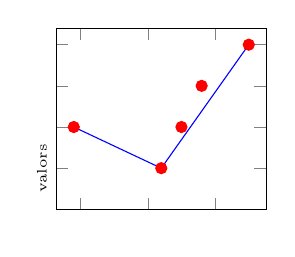
\begin{tikzpicture}
      \begin{axis}[
        % width=10cm,
        scale only axis, height=2.3cm,
        ymin = 0,
        yticklabels= {,,\tiny valors},
        y tick label style = {rotate=90,anchor=south},
        xticklabels={,{\tiny temps}},
        ]
 
        \addplot[only marks,mark=*,red] coordinates {
          (19,4)
          (32,2)
          (35,4)
          (38,6)
          (45,8)
        };

        \addplot[blue] coordinates {
          (19,4)
          (32,2)
          (45,8)
        };

    \end{axis}
  \end{tikzpicture}

  

  \column{6cm}
  \centering
  Repr.\ \emph{zero-order hold} cap enrere
  
  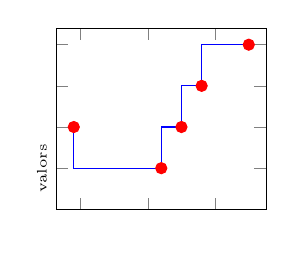
\begin{tikzpicture}
    \begin{axis}[
      % width=10cm,
      scale only axis, height=2.3cm,
      ymin = 0,
      yticklabels= {,,\tiny valors},
      y tick label style = {rotate=90,anchor=south},
      xticklabels={,{\tiny temps}},
      ]
      
      \addplot[only marks,mark=*,red] coordinates {
        (19,4)
        (32,2)
        (35,4)
        (38,6)
        (45,8)
      };
      
      
      \addplot[blue,const plot mark right] coordinates {
        (19,4)
        (32,2)
        (35,4)
        (38,6)
        (45,8)
      };
      
    \end{axis}
  \end{tikzpicture}

\end{columns}
\end{frame}



\begin{frame}{Model RRD: interpolació de sèries temporals}

  \begin{center}
  \textbf{Interpolador}: Sèrie temporal $\times$ interval de temps
  $\rightarrow$ Mesura
  \end{center}

  \vfill

  \begin{columns}[l]
    \column{.60\textwidth}
    Sèrie temporal $S$, amb $S(t)$ repr.\ \emph{zoh} cap enrere:\medskip
    
    Interpolador:  $S \times$ $[t_{i-1}^N , t_i^N] \mapsto m' = (v',t_i^N)$

    \begin{itemize}

    \item  Mitjana: 
      $$v' = \text{avg }\{V(m): m \in S(t_{i-1}^N,t_i^N]\}$$
    \item  Àrea:
      $$v' = \frac{\int_{t_{i-1}^N}^{t_i^N} S(t)dt}{t_i^N - t_{i-1}^N}$$

    \end{itemize}

    \column{.40\textwidth}
     
    \begin{center}
      \scriptsize
      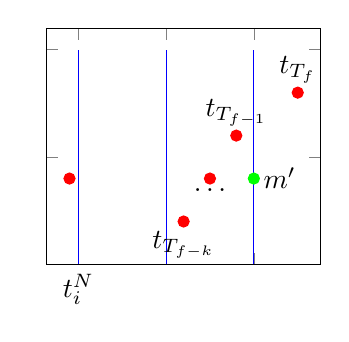
\begin{tikzpicture}
        \begin{axis}[
          % width=10cm,
          scale only axis, height=3cm,
          ymin = 0,
          yticklabels= {},
          xticklabels={$\ldots$,$t_{i-1}^N$,$t_i^N$},
          ]
          \addplot[ycomb,blue] coordinates {
            (20,10)
            (30,10)
            (40,10)
          }; 
          
          \addplot[only marks,mark=*,red] coordinates {
            (19,4)
            (32,2)
            (35,4)
            (38,6)
            (45,8)
          };
          
          \addplot[only marks,mark=*,green] coordinates {
            (40,4)
          };
          
          
          \node[below] at (axis cs:32,2) {$t_{T_{f-k}}$};
          \node[below] at (axis cs:35,4) {$\ldots$};
          \node[above] at (axis cs:38,6) {$t_{T_{f-1}}$};
          \node[above] at (axis cs:45,8) {$t_{T_f}$};
          \node[right] at (axis cs:40,4) {$m'$};
        \end{axis}
      \end{tikzpicture}
    \end{center}
  \end{columns}
\end{frame}


%%% Local Variables: 
%%% mode: latex
%%% TeX-master: "presentacio"
%%% End: 
